% =============================================================================
%  The assumptions of a one-dimensional PBL closure, as a pyramid -- VERTICAL version
%  GENERATED by scripts/make_pyramid_vertical.py from pbl_assumptions_pyramid_split.tex; edit the
%  horizontal file and regenerate. Tiers are columns (physics | concepts | formalism); a block
%  touches at its left exactly what it relies on. Scale: 0.86 cm per old cm along the ground,
%  column widths [2.5, 4.18, 5.3] cm for premises, concepts, formalism. Build: tectonic pbl_assumptions_pyramid_vertical.tex
% =============================================================================
\documentclass[10pt]{article}
\usepackage{iftex}
\ifPDFTeX
  \usepackage[utf8]{inputenc}
  \usepackage[T1]{fontenc}
  \usepackage{lmodern}
\else
  \usepackage{fontspec}
  \setmainfont{lmroman10-regular.otf}[BoldFont=lmroman10-bold.otf,
    ItalicFont=lmroman10-italic.otf, BoldItalicFont=lmroman10-bolditalic.otf]
\fi
\usepackage[british]{babel}
\usepackage[a4paper,margin=9mm,top=9mm,bottom=9mm]{geometry}
\usepackage{amsmath,amssymb}
\usepackage{xcolor}
\usepackage{tikz}
\usepackage{microtype}
\pagestyle{empty}
\setlength{\parindent}{0pt}
\setlength{\parskip}{0.5ex}
% rigid math relation spacing: the centred block texts would otherwise stretch around = and <<
\thickmuskip=5mu \medmuskip=4mu \thinmuskip=3mu

% ---- notation ---------------------------------------------------------------
\newcommand{\avg}[1]{\langle #1 \rangle}
\newcommand{\pd}[2]{\partial #1/\partial #2}
\newcommand{\qsq}{q^{2}}
\newcommand{\Rfc}{R_{fc}}
\newcommand{\dx}{\Delta x}
% ---- rows the PhD concept turns on (same data as the note's macros.tex) ------
\definecolor{cKey}{HTML}{7B2D8E}
\definecolor{cGXIX}{HTML}{990011}   % Goger 2019 port (the note's colour)
\definecolor{cFULL}{HTML}{7B2D8E}   % Kosovic-Juliano 3D closure (the note's colour)
% \hl{x0}{x1}{y0}{y1}{colour}{inset}: a frame inside a block, marking a scheme's decisive block
\newcommand{\hl}[6]{\draw[#5, line width=1.1pt] (#1+#6,#3+#6) rectangle (#2-#6,#4-#6);}
\newcommand{\setkey}[2]{\expandafter\def\csname key@#1\endcsname{#2}}
\makeatletter
\setkey{A1}{1}\setkey{B1}{1}\setkey{B2}{1}\setkey{B3}{1}\setkey{C3}{1}\setkey{C4}{1}\setkey{C6}{1}\setkey{C7}{1}
\setkey{B5}{2}\setkey{B6}{2}\setkey{C2}{2}\setkey{C5}{2}\setkey{C9}{2}
\newcommand{\keymark}[1]{\ifcsname key@#1\endcsname
  \if1\csname key@#1\endcsname\textcolor{cKey}{$\blacktriangleright$}\else\textcolor{cKey}{$\triangleright$}\fi\fi}
\makeatother
\newcommand{\pid}[1]{\keymark{#1}\textbf{#1}}
% \pb{x0}{x1}{y0}{y1}{style}{text}: a block from (x0,y0) to (x1,y1), text centred
\newcommand{\pbf}[7]{\pgfmathsetmacro{\pbw}{#2-#1-#7}%
  \draw[#5] (#1,#3) rectangle (#2,#4);
  \node[align=center, font=\tiny, inner sep=0pt, text width=\pbw cm] at ({(#1+#2)/2},{(#3+#4)/2}) {#6};}
% \pbunion{style}{tx}{ty}{tw}{text}{pieces x0/x1/y0/y1,...}{outline (x,y) -- ...}: one block of several rectangles
\newcommand{\pbunion}[7]{\foreach \ux/\uX/\uy/\uY in {#6} {\fill[black!22] (\ux,\uy) rectangle (\uX,\uY);}
  \draw[#1, fill=none] #7 -- cycle;
  \node[align=center, font=\tiny, inner sep=0pt, text width=#4 cm] at (#2,#3) {#5};}
\newcommand{\pb}[6]{\pgfmathsetmacro{\pbw}{#2-#1-0.20}%
  \draw[#5] (#1,#3) rectangle (#2,#4);
  \node[align=center, font=\tiny, inner sep=0pt, text width=\pbw cm] at ({(#1+#2)/2},{(#3+#4)/2}) {#6};}


% ---- the hectometre-scale column (used by the VERTICAL version only; read by scripts/make_pyramid_vertical.py)
% \hecto{<formal statement title>}{<what becomes of it at Delta = 500 m over the Inn Valley>}; no-op here.
% Sources: the mountain and grey-zone columns of the note's Table I.1 and the project's own runs.
\newcommand{\hecto}[2]{}
\hecto{Grid means are ensemble means}{By day, the largest eddies (of size $z_i$) are partly resolved, so the grid mean is no longer an ensemble mean. The shear of these eddies then enters both the resolved and the subgrid production. At night, all eddies are far smaller than $\dx$ again.}
\hecto{Column approximation}{Across the valley, the jet's horizontal shear is a sizeable fraction of its vertical shear.}
\hecto{Vertical divergence only}{Horizontal flux divergences are as large as the vertical one; valley budgets close only with horizontal transport and advection.}
\hecto{Wall value of $\qsq$}{At night, the turbulence near the ground hinges on the wall value; the $u_*$ of the sonics gives an observed one to test it.}
\hecto{Level-2.5 truncation}{Valid in stable and weakly unstable air, not in free convection. In fast transitions, the flow changes faster than the eddies adjust.}
\hecto{Stability functions}{No scheme we compare switches the turbulence off at a critical Richardson number. In stable air, all schemes but 3d-full take $S_M$ and $S_H$ from the vertical gradients alone.}
\hecto{Surface fluxes and first level}{The first model level is no longer in a constant-flux layer: the katabatic jet maximum lies below it, and over forest it lies in the roughness sublayer.}
\hecto{Master length scale}{In a valley, neither $z_i$ nor the wall distance is well defined, and the horizontal eddies are limited by the valley width: one length is not enough.}
\hecto{Constant set}{The constants were fitted to flat, dry boundary layers; whether they hold in valley flows is untested.}
\hecto{One length for $K$ and $\varepsilon$}{The dissipation does not depend on the grid, whereas the subgrid energy does. For this reason, the dissipation length has to shrink with $\dx$.}
\hecto{Pressure terms}{Taking them as small is a strong assumption in complex terrain, and only the residual of a measured TKE budget can test it.}
\hecto{K-form fluxes}{By day, plumes carry heat partly against the local gradient. Where slope and valley winds meet, the stress may leave the direction of the shear.}
\hecto{Buoyancy term}{On a slope, the surface heat flux has a horizontal component that a purely vertical buoyancy term misses.}

% ---- dependencies the contact rule cannot draw (post-audit list; used by scripts/make_pyramid_graph.py). No-op here.
\newcommand{\lean}[3][2]{}  % \lean[weight]{child}{parent}; weight 3 load-bearing, 2 real (default), 1 bookkeeping
% grouped by child; the order within a child is the importance of the parent (2026-09-21, Elias): the colour page
% draws the first three of weight >= 2 as corner marks, bottom left first, then counter-clockwise; the block's text names the same.
% Weights (Elias 2026-09-21): 3 load-bearing (thick border), 2 real, 1 bookkeeping (listed, not drawn).
\lean[2]{Boundary-layer approximation}{Boussinesq}
\lean[3]{Energy cascade}{Stationarity}
\lean[2]{Energy cascade}{Mixing}
\lean[2]{Local equilibrium}{Locality}
\lean[2]{Local equilibrium}{Horizontal homogeneity}
\lean[2]{Monin--Obukhov similarity}{Horizontal homogeneity}
\lean[2]{Monin--Obukhov similarity}{Constant-flux layer}
\lean[2]{Mixing length}{Horizontal homogeneity}
\lean[2]{Mixing length}{Mixing}
\lean[2]{Locality}{Mixing}
\lean[2]{Eddy viscosity}{Mixing length}
\lean[1]{Eddy viscosity}{Locality}
\lean[2]{Return to isotropy}{Horizontal homogeneity}
\lean[3]{Stability functions}{Local equilibrium}
\lean[3]{Stability functions}{Buoyancy production}
\lean[2]{Stability functions}{Boundary-layer approximation}
\lean[1]{Stability functions}{Level-2.5 truncation}
\lean[1]{Stability functions}{Universal constants}
\lean[2]{Level-2.5 truncation}{Weak anisotropy}
\lean[2]{Buoyancy production}{Return to isotropy}
\lean[1]{Universal constants}{Reynolds decomposition}
\lean[1]{Vertical divergence only}{Spectral gap}
\lean[1]{Wall value of $\qsq$}{Universal constants}
\lean[3]{Master length scale}{Buoyancy term}
\lean[3]{Buoyancy term}{K-form fluxes}
\lean[1]{Pressure terms}{Universal constants}
\lean[1]{Pressure terms}{Locality}
\lean[3]{One length for $K$ and $\varepsilon$}{Master length scale}
\lean[3]{K-form fluxes}{Master length scale}
\lean[3]{K-form fluxes}{Stability functions}
% ---- scheme quicklook (moons above the formalism tier; scripts/make_moons.py rewrites the strip)
% \moon{<block title>}{K|P|D x4} in the order MYNN as run, G19 port, 3D-APPROX, 3D-FULL; from Table I.0 of the note:
% a block is K if all its rows are kept, D if all are dropped, else P. No-op here (data only).
\newcommand{\moon}[2]{}
\moon{Grid means are ensemble means}{P K P P}
\moon{Column approximation}{K P K D}
\moon{Vertical divergence only}{P P P D}   % MYNN P since 2026-10-26: the control advects TKE (Table 1 of the concept)
\moon{Wall value of $\qsq$}{K K D D}
\moon{Level-2.5 truncation}{K K K K}
\moon{Stability functions}{K P K D}   % 2026-10-26 (Elias): level-2.5 block, no cutoff in any scheme; G19 half (its HSP source knows no Ri), 3D-FULL has no S_M, S_H
\moon{Surface fluxes and first level}{K K K K}
\moon{Master length scale}{K P K K}
\moon{Constant set}{K K K K}
\moon{One length for $K$ and $\varepsilon$}{K K K K}
\moon{Pressure terms}{K K K K}
\moon{K-form fluxes}{K P P D}   % MYNN K since 2026-10-26: the control runs without mass flux (bl_mynn_edmf = 0)
\moon{Buoyancy term}{P P P P}
% glyphs (the note's), absolute size, colour = scheme identity
\newcommand{\gK}{\tikz[baseline=-0.6ex]{\fill (0,0) circle (0.11);}}
\newcommand{\gP}{\tikz[baseline=-0.6ex]{\draw[line width=0.5pt] (0,0) circle (0.11); \fill (0,0) -- (90:0.11) arc (90:270:0.11) -- cycle;}}
\newcommand{\gD}{\tikz[baseline=-0.6ex]{\draw[line width=0.5pt] (0,0) circle (0.11);}}
\definecolor{cMYNN}{HTML}{3A6B00}    % MYNN as run
\definecolor{cAPPROX}{HTML}{9A5AA8}  % 3D-APPROX


% vertical block: rectangle + centred text, text width = block width - hpad
\newcommand{\pbv}[7]{\pgfmathsetmacro{\pbw}{#2-#1-#7}%
  \draw[#5] (#1,#3) rectangle (#2,#4);
  \node[align=center, font=\fontsize{7}{7.5}\selectfont, inner sep=0pt, text width=\pbw cm] at ({(#1+#2)/2},{(#3+#4)/2}) {#6};}
\newcommand{\hlv}[6]{\draw[#5, line width=1.1pt] (#1+#6,#3+#6) rectangle (#2-#6,#4-#6);}
% compound blocks in the page's text size
\renewcommand{\pbunion}[7]{\foreach \ux/\uX/\uy/\uY in {#6} {\fill[black!22] (\ux,\uy) rectangle (\uX,\uY);}
  \draw[#1, fill=none] #7 -- cycle;
  \node[align=center, font=\fontsize{7}{7.5}\selectfont, inner sep=0pt, text width=#4 cm] at (#2,#3) {#5};}
% hectometre box: dashed, left-aligned commentary beside a concept (not a block of the chain)
\newcommand{\pbh}[5]{\pgfmathsetmacro{\pbw}{#2-#1-0.30}%
  \draw[hecto] (#1,#3) rectangle (#2,#4);
  \node[align=left, font=\fontsize{6.5}{7.6}\selectfont, inner sep=0pt, text width=\pbw cm] at ({(#1+#2)/2},{(#3+#4)/2}) {#5};}

\begin{document}
{\large\bfseries The assumptions of a one-dimensional PBL closure, as a pyramid: what rests on what}\\[0.2ex]
{\small Vertical page of the split variant: spectral gap and gradient scale as separate premises. 2026-09-17.}

\vspace{0.3ex}
{\footnotesize Left, dark grey: the premises, hypotheses about the fluid and the flow. Middle, light grey: the concepts of
turbulence theory that follow. White: the formal statements of the level-2.5 closure. A block touches at its left
exactly the blocks it relies on; blocks in one column do not touch. Frames: \textcolor{cGXIX}{\textbf{red}} the Goger 2019
port, \textcolor{cFULL}{\textbf{purple}} the Kosovi\'c--Juliano three-dimensional closure, nested both. Right of the
formalism, dashed: what becomes of each formal statement in hectometre-scale simulations over complex terrain, here
$\Delta = 500$~m in the Inn Valley.
Far right, the concept's four schemes, left to right \textcolor{cMYNN}{\textbf{MYNN as
run}}, \textcolor{cGXIX}{\textbf{G19 port}}, \textcolor{cAPPROX}{\textbf{3D-APPROX}}, \textcolor{cFULL}{\textbf{3D-FULL}}:
\gK{} the scheme as run implements the statement, \gP{} partly, \gD{} drops it. Rules and reading on the next page.\par}

\vspace{0.4ex}
\begin{center}
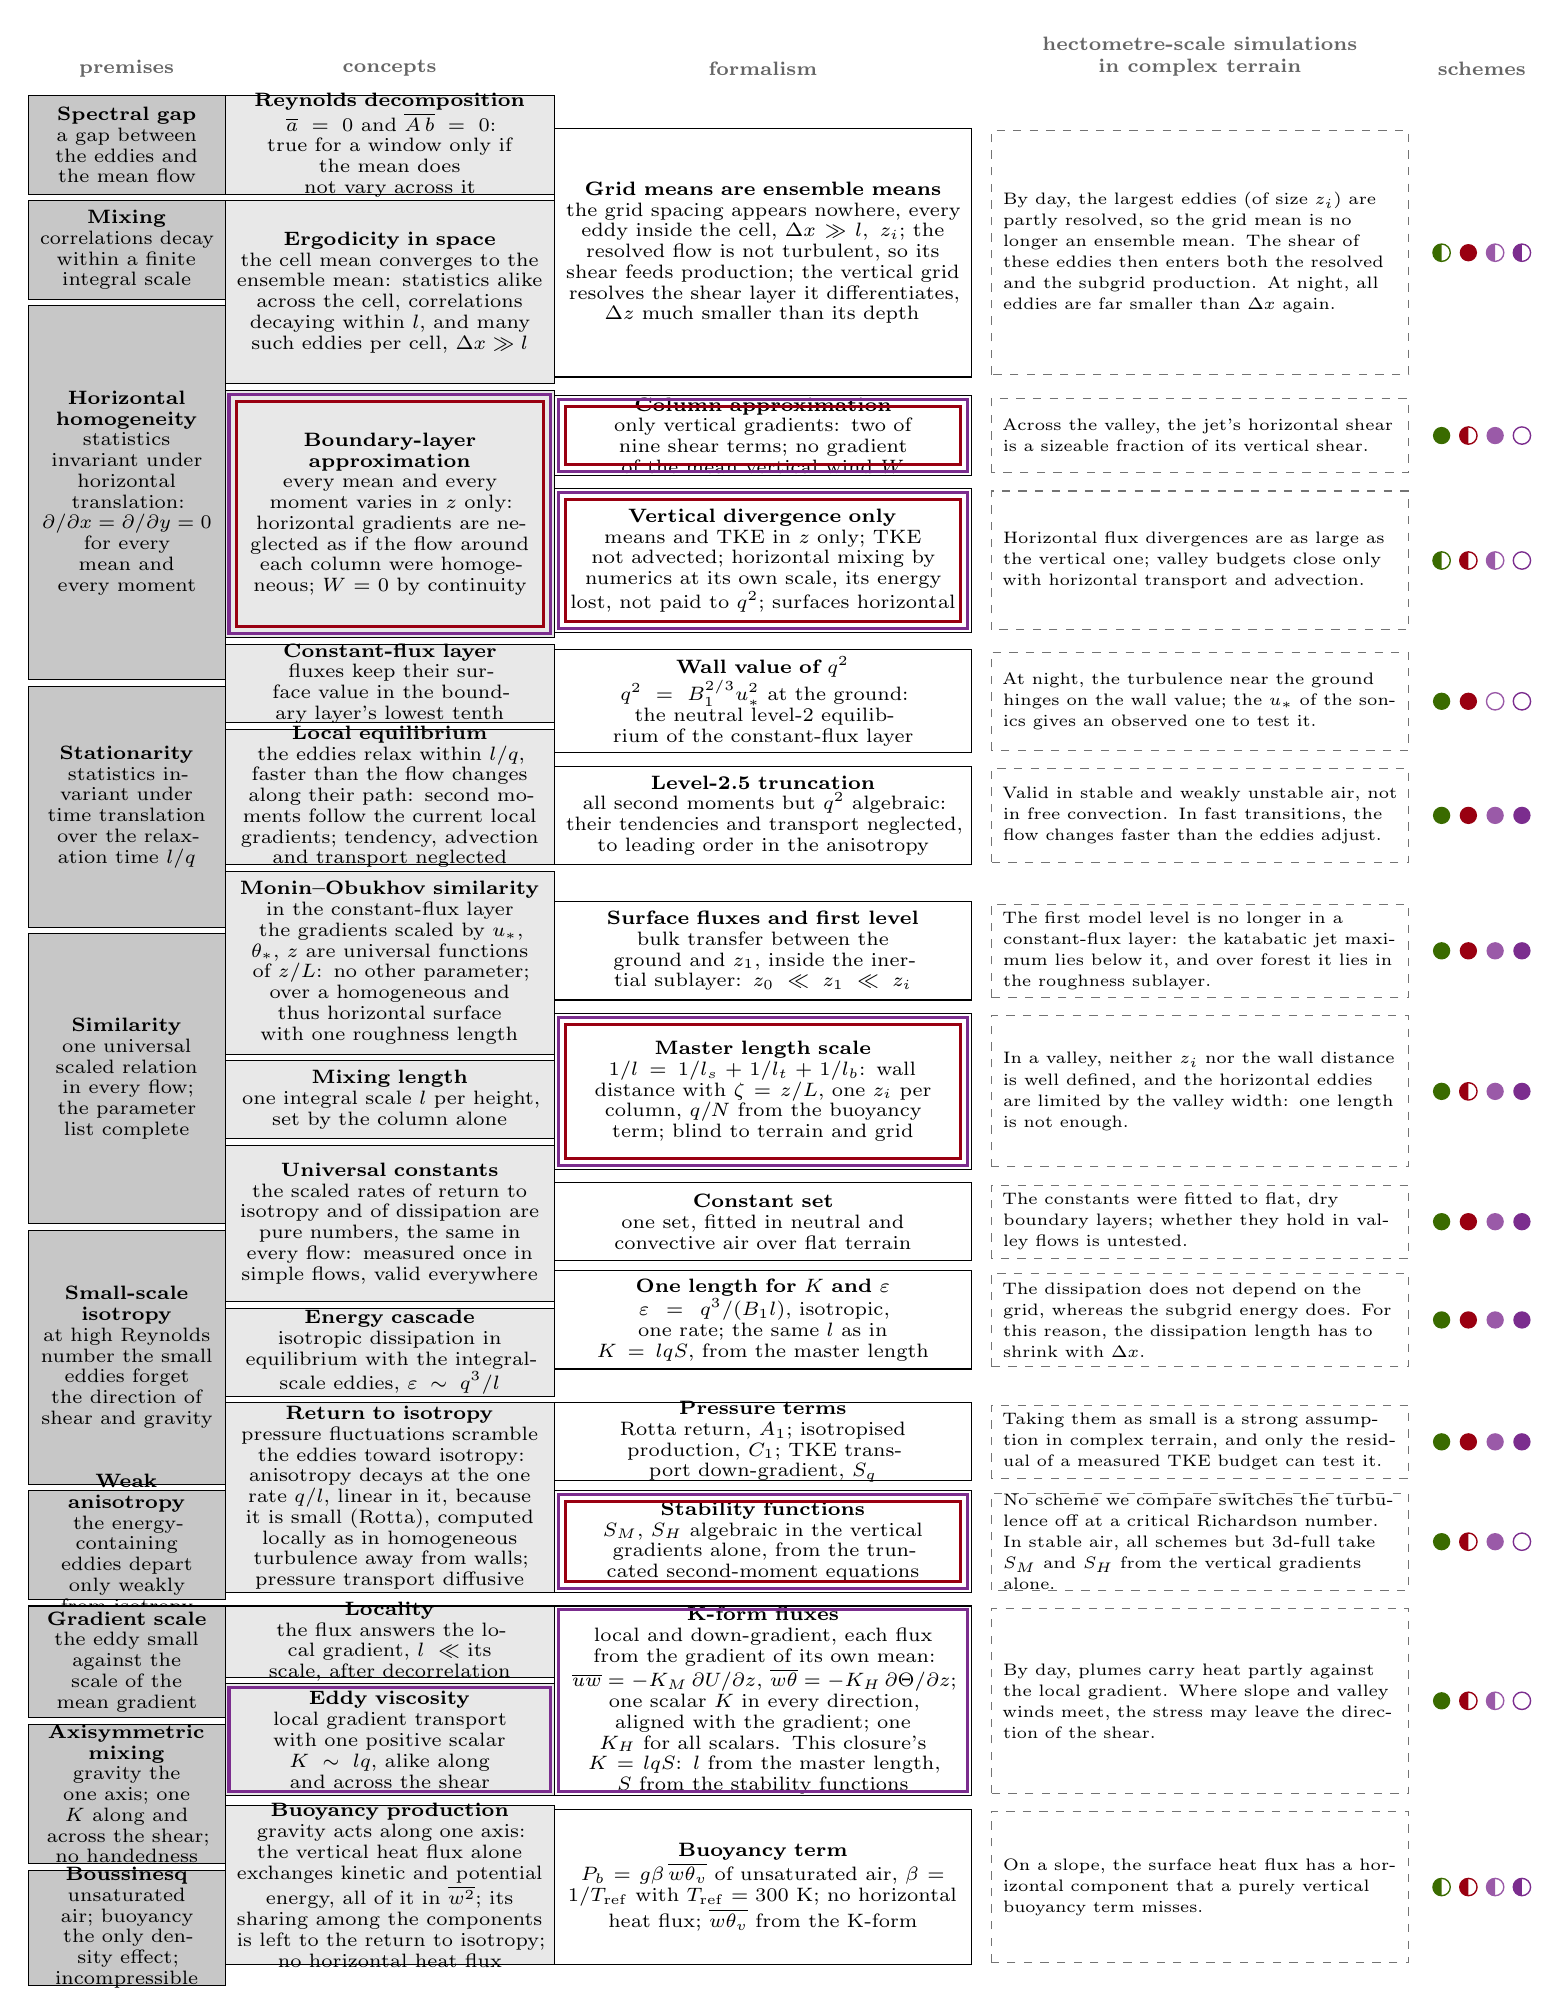
\begin{tikzpicture}[x=1cm, y=1cm,
  ground/.style={draw, line width=0.4pt, fill=black!22},
  hyp/.style={draw, line width=0.4pt, fill=black!9},
  row/.style={draw, line width=0.4pt, fill=white},
  hecto/.style={draw=black!55, dashed, line width=0.4pt, fill=white}]
\node[font=\scriptsize\bfseries, text=black!60] at (1.250,23.871) {premises};
\node[font=\scriptsize\bfseries, text=black!60] at (4.590,23.871) {concepts};
\node[font=\scriptsize\bfseries, text=black!60] at (9.330,23.871) {formalism};
\node[font=\scriptsize\bfseries, text=black!60] at (18.460,23.871) {schemes};
\node[font=\scriptsize\bfseries, text=black!60, align=center] at (14.880,24.021) {hectometre-scale simulations\\ in complex terrain};
\pbv{0.000}{2.500}{22.274}{23.521}{ground}{\textbf{Spectral gap}\\ a gap between the eddies and the mean flow}{0.30}
\pbv{0.000}{2.500}{20.941}{22.188}{ground}{\textbf{Mixing}\\ correlations decay within a finite integral scale}{0.30}
\pbv{0.000}{2.500}{12.965}{16.018}{ground}{\textbf{Stationarity}\\ statistics invariant under time translation over the relaxation time $l/q$}{0.30}
\pbv{0.000}{2.500}{9.202}{12.879}{ground}{\textbf{Similarity}\\ one universal scaled relation in every flow; the parameter list complete}{0.30}
\pbv{0.000}{2.500}{16.104}{20.855}{ground}{\textbf{Horizontal homogeneity}\\ statistics invariant under horizontal translation: \mbox{$\partial/\partial x = \partial/\partial y = 0$} for every mean and every moment}{0.30}
\pbv{0.000}{2.500}{5.891}{9.116}{ground}{\textbf{Small-scale isotropy}\\ at high Reynolds number the small eddies forget the direction of shear and gravity}{0.30}
\pbv{0.000}{2.500}{4.429}{5.805}{ground}{\textbf{Weak anisotropy}\\ the energy-containing eddies depart only weakly from isotropy}{0.30}
\pbv{0.000}{2.500}{2.924}{4.343}{ground}{\textbf{Gradient scale}\\ the eddy small against the scale of the mean gradient}{0.30}
\pbv{0.000}{2.500}{1.075}{2.838}{ground}{\textbf{Axisymmetric mixing}\\ gravity the one axis; one $K$ along and across the shear; no handedness}{0.30}
\pbv{0.000}{2.500}{-0.473}{0.989}{ground}{\textbf{Boussinesq}\\ unsaturated air; buoyancy the only density effect; incompressible}{0.30}
\pbv{2.500}{6.680}{22.274}{23.521}{hyp}{\textbf{Reynolds decomposition}\\ $\overline{a} = 0$ and $\overline{A\,b} = 0$:\\ true for a window only if\\ the mean does not vary across it}{0.30}
\pbv{2.500}{6.680}{19.866}{22.188}{hyp}{\textbf{Ergodicity in space}\\ the cell mean converges to the ensemble mean: statistics alike across the cell, correlations decaying within $l$, and many such eddies per cell, \mbox{$\dx \gg l$}}{0.30}
\pbv{2.500}{6.680}{16.641}{19.780}{hyp}{\textbf{Boundary-layer approximation}\\ every mean and every moment varies in $z$ only: horizontal gradients are neglected as if the flow around each column were homogeneous; $W = 0$ by continuity}{0.56}
\pbv{2.500}{6.680}{15.566}{16.555}{hyp}{\textbf{Constant-flux layer}\\ fluxes keep their surface value in the boundary layer's lowest tenth}{0.30}
\pbv{2.500}{6.680}{13.760}{15.480}{hyp}{\textbf{Local equilibrium}\\ the eddies relax within $l/q$, faster than the flow changes along their path: second moments follow the current local gradients; tendency, advection and transport neglected}{0.30}
\pbv{2.500}{6.680}{11.352}{13.674}{hyp}{\textbf{Monin--Obukhov similarity}\\ in the constant-flux layer the gradients scaled by $u_*$, $\theta_*$, $z$ are universal functions of $z/L$: no other parameter; over a homogeneous and thus horizontal surface with one roughness length}{0.30}
\pbv{2.500}{6.680}{10.277}{11.266}{hyp}{\textbf{Mixing length}\\ one integral scale $l$ per height, set by the column alone}{0.30}
\pbv{2.500}{6.680}{8.213}{10.191}{hyp}{\textbf{Universal constants}\\ the scaled rates of return to isotropy and of dissipation are pure numbers, the same in every flow: measured once in simple flows, valid everywhere}{0.30}
\pbv{2.500}{6.680}{7.009}{8.127}{hyp}{\textbf{Energy cascade}\\ isotropic dissipation in equilibrium with the integral-scale eddies, $\varepsilon \sim q^3/l$}{0.30}
\pbv{2.500}{6.680}{4.515}{6.923}{hyp}{\textbf{Return to isotropy}\\ pressure fluctuations scramble the eddies toward isotropy: anisotropy decays at the one rate $q/l$, linear in it, because it is small (Rotta), computed locally as in homogeneous turbulence away from walls; pressure transport diffusive}{0.30}
\pbv{2.500}{6.680}{1.935}{3.354}{hyp}{\textbf{Eddy viscosity}\\ local gradient transport with one positive scalar $K \sim l q$, alike along and across the shear}{0.40}
\pbv{2.500}{6.680}{3.440}{4.343}{hyp}{\textbf{Locality}\\ the flux answers the local gradient, $l \ll$ its scale, after decorrelation}{0.30}
\pbv{2.500}{6.680}{-0.215}{1.806}{hyp}{\textbf{Buoyancy production}\\ gravity acts along one axis: the vertical heat flux alone exchanges kinetic and potential energy, all of it in $\overline{w^2}$; its sharing among the components is left to the return to isotropy; no horizontal heat flux}{0.30}
\pbv{6.680}{11.980}{19.952}{23.108}{row}{\textbf{Grid means are ensemble means}\\ the grid spacing appears nowhere, every eddy inside the cell, $\dx \gg l,\ z_i$; the resolved flow is not turbulent, so its shear feeds production; the vertical grid resolves the shear layer it differentiates, $\Delta z$ much smaller than its depth}{0.30}
\pbv{6.680}{11.980}{18.705}{19.711}{row}{\textbf{Column approximation}\\ only vertical gradients: two of nine shear terms; no gradient of the mean vertical wind $W$}{0.56}
\pbv{6.680}{11.980}{16.710}{18.533}{row}{\textbf{Vertical divergence only}\\ means and TKE in $z$ only; TKE not advected; horizontal mixing by numerics at its own scale, its energy lost, not paid to $\qsq$; surfaces horizontal}{0.40}
\pbv{6.680}{11.980}{15.179}{16.486}{row}{\textbf{Wall value of $\qsq$}\\ $\qsq = B_1^{2/3} u_*^2$ at the ground: the neutral level-2 equilibrium of the constant-flux layer}{0.30}
\pbv{6.680}{11.980}{13.760}{15.007}{row}{\textbf{Level-2.5 truncation}\\ all second moments but $\qsq$ algebraic: their tendencies and transport neglected, to leading order in the anisotropy}{0.30}
\pbv{6.680}{11.980}{12.040}{13.287}{row}{\textbf{Surface fluxes and first level}\\ bulk transfer between the ground and $z_1$, inside the inertial sublayer: $z_0 \ll z_1 \ll z_i$}{0.30}
\pbv{6.680}{11.980}{9.890}{11.868}{row}{\textbf{Master length scale}\\ $1/l = 1/l_s + 1/l_t + 1/l_b$: wall distance with $\zeta = z/L$, one $z_i$ per column, $q/N$ from the buoyancy term; blind to terrain and grid}{0.56}
\pbv{6.680}{11.980}{8.729}{9.718}{row}{\textbf{Constant set}\\ one set, fitted in neutral and convective air over flat terrain}{0.30}
\pbv{6.680}{11.980}{7.353}{8.600}{row}{\textbf{One length for $K$ and $\varepsilon$}\\ $\varepsilon = q^3/(B_1 l)$, isotropic, one rate; the same $l$ as in $K = lqS$, from the master length}{0.30}
\pbv{6.680}{11.980}{5.934}{6.923}{row}{\textbf{Pressure terms}\\ Rotta return, $A_1$; isotropised production, $C_1$; TKE transport down-gradient, $S_q$}{0.30}
\pbv{6.680}{11.980}{4.515}{5.805}{row}{\textbf{Stability functions}\\ $S_M$, $S_H$ algebraic in the vertical gradients alone, from the truncated second-moment equations}{0.56}
\pbv{6.680}{11.980}{1.935}{4.343}{row}{\textbf{K-form fluxes}\\ local and down-gradient, each flux from the gradient of its own mean: \mbox{$\overline{uw} = -K_M\,\partial U/\partial z$}, \mbox{$\overline{w\theta} = -K_H\,\partial\Theta/\partial z$}; one scalar $K$ in every direction, aligned with the gradient; one $K_H$ for all scalars. This closure's $K = lqS$: $l$ from the master length, $S$ from the stability functions}{0.40}
\pbv{6.680}{11.980}{-0.215}{1.763}{row}{\textbf{Buoyancy term}\\ $P_b = g\beta\,\overline{w\theta_v}$ of unsaturated air, $\beta = 1/T_\mathrm{ref}$ with $T_\mathrm{ref} = 300$~K; no horizontal heat flux; $\overline{w\theta_v}$ from the K-form}{0.30}
\hlv{2.500}{6.680}{16.641}{19.780}{cFULL}{0.05}
\hlv{2.500}{6.680}{16.641}{19.780}{cGXIX}{0.14}
\hlv{6.680}{11.980}{18.705}{19.711}{cFULL}{0.05}
\hlv{6.680}{11.980}{18.705}{19.711}{cGXIX}{0.14}
\hlv{6.680}{11.980}{16.710}{18.533}{cFULL}{0.05}
\hlv{6.680}{11.980}{16.710}{18.533}{cGXIX}{0.14}
\hlv{6.680}{11.980}{4.515}{5.805}{cFULL}{0.05}
\hlv{6.680}{11.980}{4.515}{5.805}{cGXIX}{0.14}
\hlv{6.680}{11.980}{9.890}{11.868}{cFULL}{0.05}
\hlv{6.680}{11.980}{9.890}{11.868}{cGXIX}{0.14}
\hlv{2.500}{6.680}{1.935}{3.354}{cFULL}{0.05}
\hlv{6.680}{11.980}{1.935}{4.343}{cFULL}{0.05}
\node[inner sep=0pt] at (17.950,21.530) {\color{cMYNN}\gP};
\node[inner sep=0pt] at (18.290,21.530) {\color{cGXIX}\gK};
\node[inner sep=0pt] at (18.630,21.530) {\color{cAPPROX}\gP};
\node[inner sep=0pt] at (18.970,21.530) {\color{cFULL}\gP};
\node[inner sep=0pt] at (17.950,19.208) {\color{cMYNN}\gK};
\node[inner sep=0pt] at (18.290,19.208) {\color{cGXIX}\gP};
\node[inner sep=0pt] at (18.630,19.208) {\color{cAPPROX}\gK};
\node[inner sep=0pt] at (18.970,19.208) {\color{cFULL}\gD};
\node[inner sep=0pt] at (17.950,17.621) {\color{cMYNN}\gP};
\node[inner sep=0pt] at (18.290,17.621) {\color{cGXIX}\gP};
\node[inner sep=0pt] at (18.630,17.621) {\color{cAPPROX}\gP};
\node[inner sep=0pt] at (18.970,17.621) {\color{cFULL}\gD};
\node[inner sep=0pt] at (17.950,15.833) {\color{cMYNN}\gK};
\node[inner sep=0pt] at (18.290,15.833) {\color{cGXIX}\gK};
\node[inner sep=0pt] at (18.630,15.833) {\color{cAPPROX}\gD};
\node[inner sep=0pt] at (18.970,15.833) {\color{cFULL}\gD};
\node[inner sep=0pt] at (17.950,14.384) {\color{cMYNN}\gK};
\node[inner sep=0pt] at (18.290,14.384) {\color{cGXIX}\gK};
\node[inner sep=0pt] at (18.630,14.384) {\color{cAPPROX}\gK};
\node[inner sep=0pt] at (18.970,14.384) {\color{cFULL}\gK};
\node[inner sep=0pt] at (17.950,12.664) {\color{cMYNN}\gK};
\node[inner sep=0pt] at (18.290,12.664) {\color{cGXIX}\gK};
\node[inner sep=0pt] at (18.630,12.664) {\color{cAPPROX}\gK};
\node[inner sep=0pt] at (18.970,12.664) {\color{cFULL}\gK};
\node[inner sep=0pt] at (17.950,10.879) {\color{cMYNN}\gK};
\node[inner sep=0pt] at (18.290,10.879) {\color{cGXIX}\gP};
\node[inner sep=0pt] at (18.630,10.879) {\color{cAPPROX}\gK};
\node[inner sep=0pt] at (18.970,10.879) {\color{cFULL}\gK};
\node[inner sep=0pt] at (17.950,9.224) {\color{cMYNN}\gK};
\node[inner sep=0pt] at (18.290,9.224) {\color{cGXIX}\gK};
\node[inner sep=0pt] at (18.630,9.224) {\color{cAPPROX}\gK};
\node[inner sep=0pt] at (18.970,9.224) {\color{cFULL}\gK};
\node[inner sep=0pt] at (17.950,7.976) {\color{cMYNN}\gK};
\node[inner sep=0pt] at (18.290,7.976) {\color{cGXIX}\gK};
\node[inner sep=0pt] at (18.630,7.976) {\color{cAPPROX}\gK};
\node[inner sep=0pt] at (18.970,7.976) {\color{cFULL}\gK};
\node[inner sep=0pt] at (17.950,6.428) {\color{cMYNN}\gK};
\node[inner sep=0pt] at (18.290,6.428) {\color{cGXIX}\gK};
\node[inner sep=0pt] at (18.630,6.428) {\color{cAPPROX}\gK};
\node[inner sep=0pt] at (18.970,6.428) {\color{cFULL}\gK};
\node[inner sep=0pt] at (17.950,5.160) {\color{cMYNN}\gK};
\node[inner sep=0pt] at (18.290,5.160) {\color{cGXIX}\gP};
\node[inner sep=0pt] at (18.630,5.160) {\color{cAPPROX}\gK};
\node[inner sep=0pt] at (18.970,5.160) {\color{cFULL}\gD};
\node[inner sep=0pt] at (17.950,3.139) {\color{cMYNN}\gK};
\node[inner sep=0pt] at (18.290,3.139) {\color{cGXIX}\gP};
\node[inner sep=0pt] at (18.630,3.139) {\color{cAPPROX}\gP};
\node[inner sep=0pt] at (18.970,3.139) {\color{cFULL}\gD};
\node[inner sep=0pt] at (17.950,0.774) {\color{cMYNN}\gP};
\node[inner sep=0pt] at (18.290,0.774) {\color{cGXIX}\gP};
\node[inner sep=0pt] at (18.630,0.774) {\color{cAPPROX}\gP};
\node[inner sep=0pt] at (18.970,0.774) {\color{cFULL}\gP};
\pbh{12.230}{17.530}{19.982}{23.078}{By day, the largest eddies (of size $z_i$) are partly resolved, so the grid mean is no longer an ensemble mean. The shear of these eddies then enters both the resolved and the subgrid production. At night, all eddies are far smaller than $\dx$ again.}
\pbh{12.230}{17.530}{18.735}{19.681}{Across the valley, the jet's horizontal shear is a sizeable fraction of its vertical shear.}
\pbh{12.230}{17.530}{16.740}{18.503}{Horizontal flux divergences are as large as the vertical one; valley budgets close only with horizontal transport and advection.}
\pbh{12.230}{17.530}{15.209}{16.456}{At night, the turbulence near the ground hinges on the wall value; the $u_*$ of the sonics gives an observed one to test it.}
\pbh{12.230}{17.530}{13.790}{14.977}{Valid in stable and weakly unstable air, not in free convection. In fast transitions, the flow changes faster than the eddies adjust.}
\pbh{12.230}{17.530}{12.070}{13.257}{The first model level is no longer in a constant-flux layer: the katabatic jet maximum lies below it, and over forest it lies in the roughness sublayer.}
\pbh{12.230}{17.530}{9.920}{11.838}{In a valley, neither $z_i$ nor the wall distance is well defined, and the horizontal eddies are limited by the valley width: one length is not enough.}
\pbh{12.230}{17.530}{8.759}{9.688}{The constants were fitted to flat, dry boundary layers; whether they hold in valley flows is untested.}
\pbh{12.230}{17.530}{7.383}{8.570}{The dissipation does not depend on the grid, whereas the subgrid energy does. For this reason, the dissipation length has to shrink with $\dx$.}
\pbh{12.230}{17.530}{5.964}{6.893}{Taking them as small is a strong assumption in complex terrain, and only the residual of a measured TKE budget can test it.}
\pbh{12.230}{17.530}{4.545}{5.775}{No scheme we compare switches the turbulence off at a critical Richardson number. In stable air, all schemes but 3d-full take $S_M$ and $S_H$ from the vertical gradients alone.}
\pbh{12.230}{17.530}{1.965}{4.313}{By day, plumes carry heat partly against the local gradient. Where slope and valley winds meet, the stress may leave the direction of the shear.}
\pbh{12.230}{17.530}{-0.185}{1.733}{On a slope, the surface heat flux has a horizontal component that a purely vertical buoyancy term misses.}
\end{tikzpicture}
\end{center}

\newpage
{\footnotesize Every block is an assumption a boundary-layer scheme makes in order to run. A block touches at its
left exactly the blocks it relies on, and blocks in one column do not touch each other. Three columns. Dark grey, the ground (left column): ten hypotheses about the fluid and the flow that rest on nothing else here; Monin--Obukhov similarity and the mixing length lean on homogeneity by text; the channel that carried it to them in earlier versions is gone (2026-09-21). Light grey, the
concepts (middle column): the constructs of turbulence theory that follow from the ground and that every closure of this family
speaks in --- the Reynolds decomposition, the boundary-layer approximation, the constant-flux layer, Monin--Obukhov similarity,
the mixing length, the eddy viscosity, Rotta's return to isotropy, Kolmogorov's cascade. White, the formalism (right column):
the statements of the level-2.5 closure as written, each resting on the concepts it applies. Each block shows its
primary reliance; the incidence matrix of the note has the full set. Where a block leans on a parent it cannot touch, its own text names that parent, as in ``$W = 0$ by continuity''; the two premises without a block, high Reynolds number and unsaturated air, are named in the premise they qualify. Not drawn, because no scheme needs them to
run: ergodicity in time and Taylor's hypothesis, which carry the observations and the calibration; the
constraints realizability and Galilean invariance, which bound the algebra rather than carry a block; and the
dynamical core's numerical dissipation. Each recorded lean carries a weight: 3 load-bearing, 2 real, 1 bookkeeping; the colour-coded page draws the first two kinds as corner marks. Scale separation appears as its two conditions, the spectral gap at the left under the averaging and the gradient scale at the right under gradient transport. The K-form stands on locality and the eddy viscosity alone, and the eddy viscosity on the gradient scale and the axisymmetry of the mixing; how this closure builds its $K = lqS$ is not part of the K-form: $l$ is the master length, $S$ the stability functions, which stand on Rotta's return, and $q$ the prognostic energy. Strict horizontal homogeneity already makes the surface horizontal, so the axisymmetry premise keeps only what homogeneity does not give: one $K$ along and across the shear. The moons at the far right are the quicklook on the four schemes of the concept's first research question, left to right \textcolor{cMYNN}{\textbf{MYNN as run}}, \textcolor{cGXIX}{\textbf{G19 port}}, \textcolor{cAPPROX}{\textbf{3D-APPROX}}, \textcolor{cFULL}{\textbf{3D-FULL}}: \gK{} the scheme as run implements the assumption, \gP{} partly, \gD{} drops it; a block takes the status of its rows in the note's Table~I.0, kept only when all are kept, dropped only when all are dropped.\par}


\vspace{0.2ex}
{\footnotesize\textbf{Frames.} The blocks each scheme's design turns on, the framed cells of the note's Table~I.0,
in the note's scheme colours. \textcolor{cGXIX}{\textbf{Red}}, the Goger 2019 port: it adds a horizontal
shear-production source to the TKE budget (column approximation), pays it with the energy the numerical
horizontal operator would otherwise lose and advects TKE (vertical divergence only), gives the source its own
horizontal length from the flow, $l_h^2 = U_h^2 T_{L,u} T_{L,v}$ (master length scale), and adds a source that knows no
Richardson number to stability functions that know only the vertical one (stability functions); at the concept level it breaks the
boundary-layer approximation for production alone and keeps every other block. \textcolor{cFULL}{\textbf{Purple}}, the
Kosovi\'c--Juliano three-dimensional closure: it drops the boundary-layer approximation entirely --- nine production
terms, three-dimensional divergences and TKE transport, metric-corrected gradients, all subgrid mixing from the
closure --- and replaces the eddy viscosity and the K-form by the solved algebraic stress tensor, so no $K$, no
alignment, no stability functions and no cutoff; the equilibrium follows from the full strain. It keeps the master
length scale, one scalar $l$ for the whole tensor: the last one-dimensional block in a three-dimensional scheme, and
the frontier. Nested frames: both schemes; the three-dimensional closure touches every block the Goger port touches and alone reaches the eddy viscosity and the K-form.\par}

\vspace{0.1ex}
{\footnotesize\textbf{Reading.} The ground holds the premises, hypotheses about the fluid and the flow; nothing in it names a model. The middle column is where
the model's vocabulary is born: the spectral gap gives the Reynolds decomposition its rules; mixing with homogeneity gives ergodicity in space; the gradient scale gives locality; homogeneity gives the
boundary-layer approximation and, with stationarity, the constant-flux layer; stationarity gives local equilibrium and, with similarity, Monin--Obukhov similarity (homogeneity by text); similarity gives the mixing length (homogeneity and mixing by text); similarity with small-scale isotropy gives universal constants; small-scale isotropy gives the cascade and, with the weak anisotropy of the energy-containing eddies, the return to isotropy; the gradient scale with the axisymmetry of the mixing gives the eddy viscosity; axisymmetric mixing and a Boussinesq fluid give buoyancy production through the vertical heat flux. The right
column is the closure as written, and every one of its statements applies one or two concepts: the truncation
applies local equilibrium; the stability functions come from Rotta's return through the truncated second-moment equations; the master length takes its wall branch from Monin--Obukhov similarity, its shape from the mixing length and its coefficients from universality;
the one-length statement takes its form from the cascade and its constant from universality; the K-form takes its locality from locality and its scalar from the eddy viscosity, and this closure's $K = lqS$ borrows $l$ from the master length and $S$ from the stability functions. Terrain breaks the ground at the top
and in the middle --- homogeneity and with it the horizontal surface, the boundary-layer approximation, the constant-flux layer --- and the grey zone breaks it
at the very top; the lower third, isotropy and its constants, no scheme in the comparison touches.\par}

\vspace{0.1ex}
{\footnotesize\textbf{Correspondence to the note's rows.} Grid means are ensemble means: A1, A2, D4. Column approximation: B1, B2. Vertical divergence only: B3, B4, B5, B7. Constant-flux layer and Monin--Obukhov similarity: the two halves of B6. Wall value of $\qsq$: the lower boundary of the TKE equation, part of B6. Surface fluxes and first level: D3 with the bulk-transfer half of B6. K-form fluxes: C1, C2, C3 and the mixing of all scalars alike. Master length scale: C4. One length for $K$ and $\varepsilon$: C5. Level-2.5 truncation: C7. Stability functions: C6 with the stability functions of C7. Buoyancy term: C8 with the dry buoyancy flux (D5). Constant set: C9. Pressure terms: C10.\par}

\end{document}
